\chapter{Rayleigh Quotient, Inverse Iteration}
In this chapter, we present some classical eigenvalue algorithms. Individually, these tools are useful in certain circumstances--especially inverse iteration, which is the standard method for determining an eigenvector when the corresponding eigenvalue is known. Combined, they are ingredients of the celebrated QR algorithm. 

\section{Restriction ot Real Symmetric Matrices}
Throughout numerical linear algebra, most algorithmic ideas are applicable either to general matrices or, with certain simplifications, to hermitian matrices. For the topics discussed in this and the next three chapters, this continues to be at least partly true, but some of the differences between the general and the hermitian cases are rather sizable. Therefore, in these four chapter, we simplify matters by considering only matrices that are real and symmetric. We also assume throughout that $\|\cdot \| = \|\cdot\|_2$.  

Thus, for these four chapters: $A= A^\top \in \RR^{m\times m}, x\in \RR^m, x^*  = x^\top , \|x\| =\sqrt{x^\top x} $. In particular, this means that $A$ has real eigenvalues and a complete set of orthogonal eigenvectors. We use the following notation: 
\begin{itemize}
    \item Real eigenvalues: $ \lambda _1, \ldots , \lambda _m $, 
    \item Orthonormal eigenvectors: $ q_1, \ldots ,q_m $.  
\end{itemize}
Most of the ideas to be described in the next few lectures pertain to Phase 2 of the two phases described in Chapter 24. This means $A$ will be tridiagonal. This tridiagonal structure is occasionally of mathematical importance, for example in choosing shifts for the QR algorithm, and it's always of algorithmic importance, reducing many steps from $O(m^3)$ to $O(m)$ flops. 

\section{Rayleigh Quotient}

%────────────────────────────────────────
\begin{definition}
[Rayleigh quotient]
\label{def: Rayleigh quotient}
The Rayleigh quotient of a vector $x\in \RR^m$ is the scalar 
\[
r(x)  = \frac{x^\top Ax}{x^\top x}.  
\] 
\end{definition}
%────────────────────────────────────────
Notice that if $x$ is an eigenvector, then $r(x) = \lambda $ is the corresponding eigenvalue. Besides, given $x$,if we want to find a scalar $\alpha $ that ``acts most like an eigenvalue'' in the sense of minimizing $\|Ax- \alpha x\|_2$, the answer should be $\alpha = r(x)$. Thus $r(x)$ is a natural eigenvalue estimate to consider if $x$ is close to, but not necessarily equal to, an eigenvector. 

Furthermore, we can compute the derivative of $r$, we have 
\[
    \frac{\partial r(x)}{\partial x_j} = \frac{\frac{\partial}{\partial x_j}(x^\top Ax)}{x^\top x} - \frac{(x^\top Ax) \frac{\partial}{\partial x_j}(x^\top x)}{(x^\top x)^2} = \frac{2(Ax)_j}{x^\top x} - \frac{(x^\top A x) 2x_j}{(x^\top x)^2} = \frac{2}{x^\top x}(Ax - r(x) x)_j.  
\]
Combine this, we get 
\[
    \nabla r(x) = \frac{2}{x^\top x}(Ax - r(x) x). 
\]
Geometrically speaking, the eigenvectors of $A$ are the stationary points of the function $r(x)$. Besides, since $r(x)$ is independent of the scale of $x$, these stationary points lie along lines through the origin in $\RR^m$. We can restrict our attention to the unit sphere $\|x\|=1$.  

%────────────────────────────────────────
\begin{figure}[H]
    \centering
    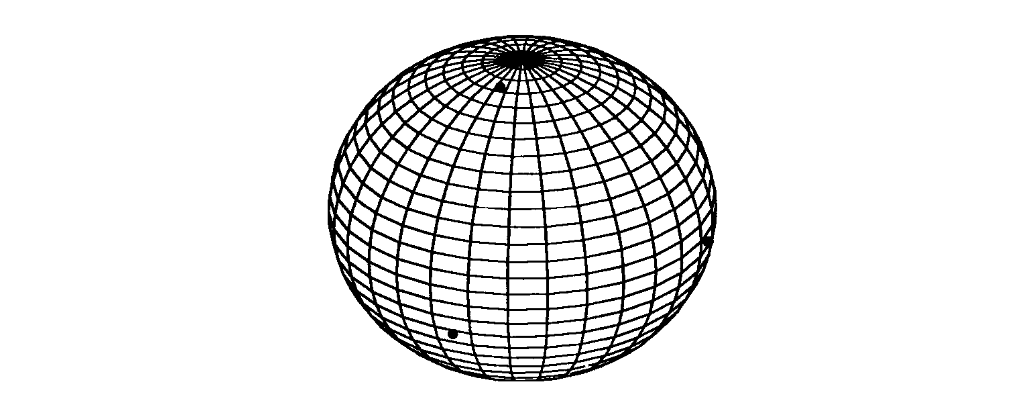
\includegraphics[width=0.8\textwidth]{figures/27-1.png}
    \caption{The Rayleigh quotient $r(x)$ is a continuous function on the unit sphere $\|x\|=1$ in $\RR^m$, and the stationary points of $r(x)$ are the normalized eigenvectors of $A$. In this example with $m=3$, there are three orthogonal stationary points. }
\end{figure}
%────────────────────────────────────────

Let $q_J$ be one of the eigenvectors of $A$. From the fact that $\nabla r(q_J) = 0$, together with the smoothness of the function $r(x)$, we derive an important consequence:
\begin{equation}
\label{eq: quadratic accurate}
r(x) - r(q_J) = O(\|x- q_J\|^2), \quad \text{ as } x \to q_J. 
\end{equation}

Thus the Rayleigh quotient is a \textbf{quadratically accurate estimate of an eigenvalue}. Herein lies its power.  

\section{Power Iteration} 
 Now we switch tacks. Suppose $v^{(0)}$ is a vector with $ \|v^{(0)}\|=1 $. The following process, \textbf{power iteration}, was cited as a not especially good idea at the beginning of Chapter 24. It may be expected to produce a sequence $ v^{s(i)} $ that converges to an eigenvector corresponding to the largest eigenvalue of $A$> 

 \begin{algorithm}[H]
     \caption{Power Iteration}
     \label{Algo 27.1}
$ v^{(0)}= $ some vector with $ \|v^{(0)}\|=1 $\; 
     \For{$ k=1,2,\ldots  $}{
        $ w = Av^{(k-1)} $\;
        $ v^{(k)}=\frac{w}{\|w\|} $\; 
        $ \lambda ^{(k)} = (v^{(k)})^\top  Av^{(k)} $\; 
     }
 \end{algorithm}
 In this and the algorithms to follow, we give no attention to termination conditions, describing the loop only by the suggestive expression. Of course, in practice, termination conditions are very important, and this is one of this points where top-quality software such as can be found in LAPACK or Matlab is likely to be superior to a program an individual might write.  

 We can analyze power iteration easily. Write $v^{(0)}$ as a linear combination of these orthonormal eigenvectors $q_i$: 
 \[
    v^{(0)} = a_1q_1 + a_2 q_2 + \cdots +a_mq_m. 
 \]
Hence, $v^{(k)}$ is: 
\begin{align*}
    v^{(k)} 
    &= c_k A^k v^{(0)}\\ 
    &= c_k (a_1 \lambda _1^k q_1 + a_2 \lambda _2^k q_2 + \cdots + a_m \lambda _m^k q_m) \\ 
    &= c_k \lambda _1^k ( a_1 q_1 + a_2 (\lambda _2 /\lambda _1)^k q_2 + \cdots + a_m (\lambda _m / \lambda _1)^k q_m),
\end{align*}
for some constants $c_k$. 


%────────────────────────────────────────
\begin{theorem}
\label{thm: convergence power iteration}
Suppose $ |\lambda _1| > |\lambda _2| \ge \cdots \ge |\lambda _m| \ge 0 $ and $q_1^\top  v^{(0)} \neq 0$. Then the iterates of Algo~\ref{Algo 27.1} satisfy 
\begin{equation}
\label{eq: convergence power iteration}
    \|v^{(k)} - (\pm q_1) \| = O\left( \left| \frac{\lambda _2}{\lambda _1} \right| ^k \right), \quad |\lambda ^{(k)} - \lambda _1| = O \left( \left| \frac{\lambda _2}{\lambda _1} \right| ^{2k} \right)   
\end{equation}
as $k\to \infty$. The $\pm$ sign, means at each step $k$, one or the other choice of sign is to be taken, and then the indicated bound holds.  
\end{theorem}
%────────────────────────────────────────
On its own, power iteration is of limited use, for several reasons. 
\begin{itemize}
    \item First, it can find only the eigenvector corresponding to the largest eigenvalue. 
    \item Second, the convergence is linear, reducing the error only by a constant factor $ \approx |\lambda _2 / \lambda _1| $ at each iteration. 
    \item Finally, the quality of this factor depends on having a largest eigenvalue that is significantly larger than the others.  
\end{itemize}
Fortunately, there is a way to amplify the differences between eigenvalues.  


\section{Inverse Iteration} 
For any $\mu\in \RR$ s.t. $\mu \notin \spec A$, we must have $E_{(\lambda-mu)^{-1} } ( (A-\mu I)^{-1})  = E_\lambda (A)$ and 
\[
    \spec (A - \mu I )^{-1}  = \{(\lambda _j -\mu)^{-1} | \lambda _j \in \spec A\}.  
\]
Suppose $\mu$ is close to an eigenvalue $\lambda _J$ of $A$. Then $(\lambda _J - \mu)^{-1} $ may be much larger than $ (\lambda _j - mu)^{-1}  $ for all $ j\neq J $. Thus, it will converge rapidly to $q_J$. This idea is called \textbf{inverse iteration}. 

\begin{algorithm}[H]
    \caption{Inverse Iteration}
    \label{Algo 27.2}
$ v^{(0)}= $ some vector with $ \|v^{(0)}\|=1 $\; 
     \For{$ k=1,2,\ldots  $}{
        Solve $(A-\mu I) w = v^{(k-1)}$ for $w$\;
        $ v^{(k)}=\frac{w}{\|w\|} $\; 
        $ \lambda ^{(k)} = (v^{(k)})^\top  Av^{(k)} $\; }
\end{algorithm}

What if $\mu$ is an eigenvalue of $A$, so that $A- \mu I$ is singular? What if it's nearly an eigenvalue, so that $ A-\mu I $ is so ill-conditioned that an accurate solution of $(A-\mu I) w = v^{(k-1)}$ cannot be expected? These cannot cause real problems. 

Like power iteration, inverse iteration exhibits only linear convergence. Unlike power iteration, however, we can choose the eigenvector that will be found by supplying an estimate $\mu$ of the corresponding eigenvalue. Furthermore, the rate of linear convergence can be controlled, for it depends on the quality of $\mu$. We have the following theorem: 


%────────────────────────────────────────
\begin{theorem}
\label{thm: convergence inverse iteration}
Suppose $ \lambda _J $ is the closest eigenvalue to $ \mu  $ and $ \lambda _K $ is the second closest, that is, $ |\mu-\lambda _J| < |\mu-\lambda _K|\le |\mu-\lambda _j| $ for each $ j\neq J $. Furthermore, suppose $ q_J^\top  v^{(0)}\neq 0 $. Then the iterates of Algo~\ref{Algo 27.2} satisfy 
\[
    \|v^{(k)}- (\pm q_J) \| = O \left( \left| \frac{\mu - \lambda _J}{\mu - \lambda _K} \right| ^k \right) , \quad |\lambda ^{(k)} - \lambda _J| = O\left( \left| \frac{\mu - \lambda _J}{\mu-\lambda _K} \right| ^{2k} \right) 
\]
as $k\to \infty$, where the $\pm$ sign has the same meaning as in Thm~\ref{thm: convergence power iteration}. 
\end{theorem}
%────────────────────────────────────────

Inverse iteration is one of the most valuable tools of NLA, for it's the standard method of calculating one or more eigenvectors of a matrix if the eigenvalues are already known.  

\section{Rayleigh Quotient Iteration} 
In this chapter, we presented two methods: one for estimating eigenvector and one for obtaining an eigenvector estimate from an eigenvalue estimate. We can combine them. 
%────────────────────────────────────────
\begin{figure}[H]
    \centering
    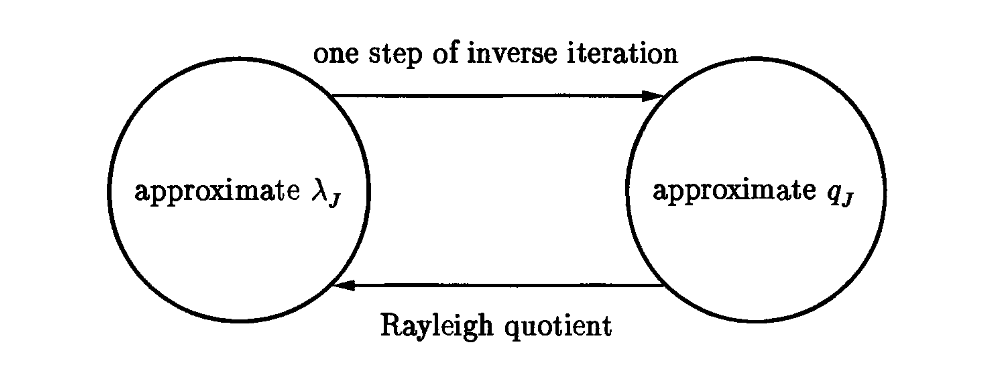
\includegraphics[width=0.8\textwidth]{figures/27-2.png}
\end{figure}
%────────────────────────────────────────

This algorithm is called \textbf{Rayleigh quotient iteration}. 

\begin{algorithm}[H]
    \caption{Rayleigh Quotient Iteration}
    \label{Algo 27.3}
    $ v^{(0)}= $ some vector with $ \|v^{(0)}\|=1 $\; 
    $ \lambda ^{(0)} = (v^{(0)})^\top  A v^{(0)} $\;
     \For{$ k=1,2,\ldots  $}{
        Solve $(A-\lambda ^{(k-1)} I) w = v^{(k-1)}$ for $w$\;
        $ v^{(k)}=\frac{w}{\|w\|} $\; 
        $ \lambda ^{(k)} = (v^{(k)})^\top  Av^{(k)} $\; }
\end{algorithm}

The convergence of this algorithm is spectacular: each iteration triples the number of digits of accuracy. 


%────────────────────────────────────────
\begin{theorem}
\label{thm: convergence rayleigh quotient}
Raleigh quotient iteration converges to an eigenvalue/eigenvector pair for all except a set of measure zero of starting vectors $v^{(0)}$. When it converges, the convergence is ultimately cubic in the sense that if $\lambda _J$ is an eigenvalue of $A$ and $v^{(0)}$ is sufficiently close to the eigenvector $q_J$, then 
\begin{equation}
\label{eq: RQ iter vector rate}
    \|v ^{(k+1)} - (\pm q_J)\| = O(\|v^{(k)} - (\pm q_J)\|^3) 
\end{equation}
and 
\begin{equation}
\label{eq: RQ iter value rate}
    |\lambda ^{(k+1)}-\lambda _J| = O(|\lambda ^{(k)}- \lambda _J|^3)
\end{equation}
as $k\to \infty$. The $ \pm $ signs are not necessarily the same on the two sides of \eqref{eq: RQ iter vector rate}. 
\end{theorem}
%────────────────────────────────────────

%────────────────────────────────────────
\begin{proof}[Proof sketch]
Firstly, we have \eqref{eq: quadratic accurate}, 
\[
    |\lambda ^{(k)} - \lambda _J|  = C \|v^{(k)} - q_J\|^2. 
\]
Then following the proof of Thm~\ref{thm: convergence inverse iteration}, 
\[
    \|v^{(k+1)}-q_J\| = O(|\lambda ^{(k)}-\lambda _J| \| v^{(k)}-q_J\|) = C \|v^{(k)}-q_J\|^3. 
\]
Similar rate can be achieved for $|\lambda ^{(k)}-\lambda _J|$. 
\end{proof}
%────────────────────────────────────────


%────────────────────────────────────────
\begin{example}
\label{eg: convergence rate eg}
Cubic convergence is so fast. Consider the symmetric matrix 
\[
    A = \begin{bmatrix}[] 
        2 & 1 &  1 \\
        1 & 3 &  1 \\
        1 & 1 &  4 \\
    \end{bmatrix},  
\]
and let $v^{(0)}=(1,1,1)^\top /\sqrt{3} $ be the initial eigenvector estimate. When Rayleigh quotient iteration is applied to $A$, the following values $ \lambda ^{(k)} $ are computed by the first three iterations: 
\[
    \lambda^{(0)}=5, \quad \lambda^{(1)}=5.2131 \ldots, \quad \lambda^{(2)}=5.214319743184 \ldots
\]
The actual value of the eigenvalue corresponding to the eigenvector closet to $v^{(0)}$ is $\lambda  = 5.414319743377$. After only three iterations, Rayleigh quotient iteration has produced a result accurate to ten digits. 
\end{example}
%────────────────────────────────────────

\section{Operation Counts}
First, suppose $A\in \RR^{m\times m}$ is a full matrix. Then each step of power iteration involves a matrix-vector multiplication, requiring $O(m^2)$ flops. Each step of inverse iteration involves the solution of a linear system, which might seem to require $O(m^3)$ flops, but this figure reduces to $O(m^2)$ if the matrix is processed in advance by LU or QR factorization or another method. In the case of Rayleigh quotient iteration, the matrix to be inverted changes at each step, and beating $O(m^3)$ flops per step is not so straightforward.  

These figures improve greatly if $A$ is tridiagonal. Now, all three iterations require just $O(m)$ flops per step. For the analogous iterations involving nonsymmetric matrices, incidentally, we must deal with Hessenberg instead of tridiagonal structure, and this figure increases to $O(m^2)$. 